\def\band{Grades K--1}\def\packet{W94-K-v4}\documentclass[letterpaper,12pt]{article}
\usepackage[margin=0.65in,headheight=18pt,headsep=18pt,footskip=24pt]{geometry}
\usepackage{tikz,array,fancyhdr,amsmath}
\usepackage[T1]{fontenc}
\usepackage{lmodern}
\renewcommand{\familydefault}{\sfdefault}
\pagestyle{fancy}\fancyhf{}
\renewcommand{\headrulewidth}{0.35pt}\renewcommand{\footrulewidth}{0pt}
\fancyhead[L]{\small Week 94 / Calibration lab / \band}
\fancyfoot[L]{\footnotesize Bellingham Math Circle / Week 94 / \packet}
\fancyfoot[R]{\footnotesize\thepage}
\setlength{\parindent}{0pt}\setlength{\parskip}{9pt}
\pdfinfoomitdate=1\pdftrailerid{}\pdfsuppressptexinfo=15
\newcommand{\problem}[2]{\par\noindent\textbf{Problem #1:} #2\par}
\newcommand{\room}[1]{\vspace{#1}}
\newcommand{\ruler}[1]{\begin{tikzpicture}[x=12mm,y=10mm]\draw[line width=.8pt] (0,0)--(12,0);\foreach \i in {0,...,12}{\draw (\i,-.13)--(\i,.13);\pgfmathtruncatemacro{\lab}{\i+#1}\node[below,font=\small] at (\i,-.15){\lab};}\end{tikzpicture}}
\newcommand{\linepair}[3]{\begin{tikzpicture}[x=9.3mm,y=8mm]\node[anchor=east,font=\normalsize] at (-.4,0){#1};\draw (0,0)--(14,0);\foreach \i in {0,...,14}{\draw (\i,-.12)--(\i,.12);\node[below,font=\scriptsize] at (\i,-.15){\i};}\fill (#2,0) circle (2.3pt);\fill (#3,0) circle (2.3pt);\end{tikzpicture}}
\newcommand{\workbox}[1]{\begin{tikzpicture}\draw[gray!55] (0,0) rectangle (16.9,#1);\end{tikzpicture}}
\newcommand{\strips}{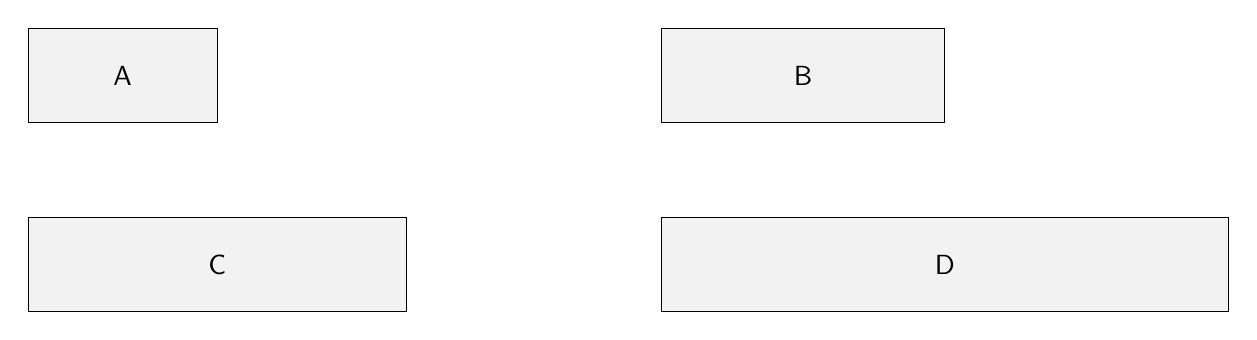
\begin{tikzpicture}[x=12mm,y=12mm]
\foreach \x/\y/\n/\s in {0/0/2/A,6.7/0/3/B,0/-2/4/C,6.7/-2/6/D}{\draw[fill=gray!10] (\x,\y) rectangle +(\n,1);\node at (\x+\n/2,\y+.5){\s};}
\end{tikzpicture}}
\newcommand{\unitrow}{\begin{tikzpicture}[x=12mm,y=12mm]\foreach\i in{0,...,11}{\draw(\i,0) rectangle +(1,1);}\end{tikzpicture}}
\newcommand{\addexample}{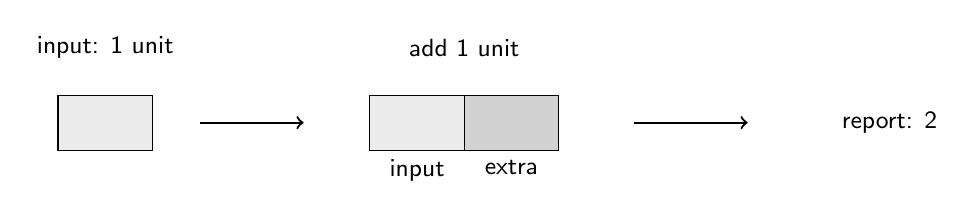
\begin{tikzpicture}[x=12mm,y=10mm,font=\small]
\node at (1.2,1.3){input: 1 unit};\draw[fill=gray!15] (.7,0) rectangle +(1,.7);
\draw[->,thick] (2.2,.35)--(3.3,.35);
\draw[fill=gray!15] (4,0) rectangle +(1,.7);\draw[fill=gray!35] (5,0) rectangle +(1,.7);
\node at (5,1.3){add 1 unit};\node[below] at (4.5,0){input};\node[below] at (5.5,0){extra};
\draw[->,thick] (6.8,.35)--(8,.35);\node at (9.5,.35){report: 2};
\end{tikzpicture}}
\newcommand{\affineexample}{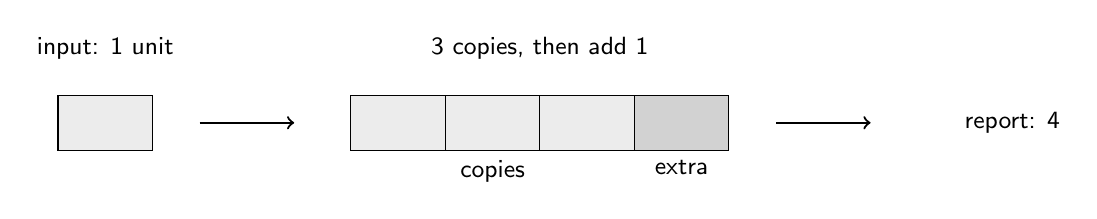
\begin{tikzpicture}[x=12mm,y=10mm,font=\small]
\node at (1,1.3){input: 1 unit};\draw[fill=gray!15] (.5,0) rectangle +(1,.7);
\draw[->,thick](2,.35)--(3,.35);
\foreach\i in{0,...,2}{\draw[fill=gray!15](3.6+\i,0)rectangle+(1,.7);}\draw[fill=gray!35](6.6,0)rectangle+(1,.7);
\node at (5.6,1.3){3 copies, then add 1};\node[below] at(5.1,0){copies};\node[below]at(7.1,0){extra};
\draw[->,thick](8.1,.35)--(9.1,.35);\node at(10.6,.35){report: 4};
\end{tikzpicture}}
\newcommand{\tcubes}[3]{\foreach\j in{1,...,#3}{\draw[fill=gray!15](#1,#2+\j-1)rectangle+(1,1);}}
\newcommand{\tcells}[3]{\foreach\j in{1,...,#3}{\draw[gray!70](#1,#2+\j-1)rectangle+(1,1);}}
\newcommand{\towerexample}{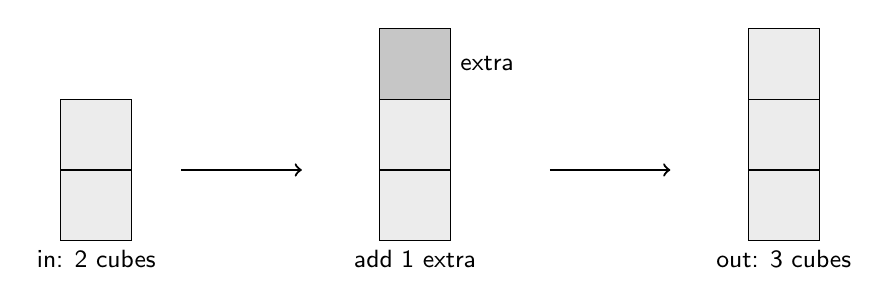
\begin{tikzpicture}[x=9mm,y=9mm,font=\small]
\tcubes{0}{0}{2}\node[below]at(.5,0){in: 2 cubes};
\draw[->,thick](1.7,1)--(3.4,1);
\tcubes{4.5}{0}{2}\draw[fill=gray!45](4.5,2)rectangle+(1,1);\node[right]at(5.5,2.5){extra};
\node[below]at(5,0){add 1 extra};
\draw[->,thick](6.9,1)--(8.6,1);
\tcubes{9.7}{0}{3}\node[below]at(10.2,0){out: 3 cubes};
\end{tikzpicture}}
\begin{document}\fontsize{15}{19}\selectfont
Use the four loose strips and the uncut row of squares. Each square is one unit. Lay strips along the ruler with both ends at printed marks.

\begin{center}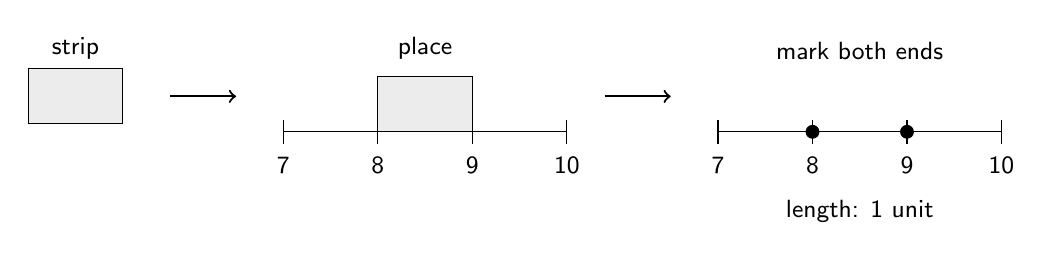
\begin{tikzpicture}[x=12mm,y=10mm,font=\small]
\draw[fill=gray!15](0,.3)rectangle(1,1);\node[above]at(.5,1){strip};
\draw[->,thick](1.5,.65)--(2.2,.65);
\draw(2.7,.2)--(5.7,.2);
\foreach\x/\n in{2.7/7,3.7/8,4.7/9,5.7/10}{\draw(\x,.05)--(\x,.35);\node[below]at(\x,0){\n};}
\draw[fill=gray!15](3.7,.2)rectangle(4.7,.9);
\node[above]at(4.2,1){place};
\draw[->,thick](6.1,.65)--(6.8,.65);
\draw(7.3,.2)--(10.3,.2);
\foreach\x/\n in{7.3/7,8.3/8,9.3/9,10.3/10}{\draw(\x,.05)--(\x,.35);\node[below]at(\x,0){\n};}
\fill(8.3,.2)circle(2.5pt);\fill(9.3,.2)circle(2.5pt);
\node[above]at(8.8,1){mark both ends};\node[below]at(8.8,-.55){length: 1 unit};
\end{tikzpicture}\end{center}

\problem{1}{How many units long is each strip? Put each strip in different places on the ruler.}

\begin{center}\ruler{2}\end{center}
\vspace{3mm}
\begin{center}\begin{tabular}{@{}p{3.6cm}p{3.6cm}p{3.6cm}p{3.6cm}@{}}A: \hrulefill&B: \hrulefill&C: \hrulefill&D: \hrulefill\end{tabular}\end{center}
\vspace{5mm}
\begin{center}\unitrow\end{center}
\vspace{5mm}
\begin{center}\strips\end{center}

\newpage

\problem{2}{Find every place each strip can go with one end at 7. Draw its two ends on a ruler.}

\begin{center}
A\quad\ruler{2}\par\vspace{3mm}
A\quad\ruler{2}\par\vspace{8mm}
B\quad\ruler{2}\par\vspace{3mm}
B\quad\ruler{2}\par\vspace{8mm}
C\quad\ruler{2}\par\vspace{3mm}
C\quad\ruler{2}\par\vspace{8mm}
D\quad\ruler{2}\par\vspace{3mm}
D\quad\ruler{2}
\end{center}
\vspace{8mm}

\problem{3}{Which two strips can you put end to end and cover exactly with a third strip? Find every way.}

\vspace{4mm}
\begin{center}\ruler{2}\end{center}

\newpage

Behind a cover, the machine takes a tower of cubes and gives back a tower with the same number of cubes plus a secret extra. A machine always adds the same extra: 1, 2 or 3 cubes.
\begin{center}\towerexample\end{center}

\problem{4}{Take turns being the machine, with your secret extra as a stick of cubes behind the cover. Your partner finds the extra; then lift the cover to check.}

\begin{center}\begin{tabular}{|p{2.6cm}|p{5.6cm}|p{5.6cm}|}\hline
Round & Towers you gave & Extra you found \\\hline
1\rule{0pt}{17mm}&&\\\hline 2\rule{0pt}{17mm}&&\\\hline 3\rule{0pt}{17mm}&&\\\hline 4\rule{0pt}{17mm}&&\\\hline
\end{tabular}\end{center}

\newpage

\problem{5}{P and Q went into the same machine: build and color every pair of towers that could have gone in. Could P be taller than Q?}

\begin{center}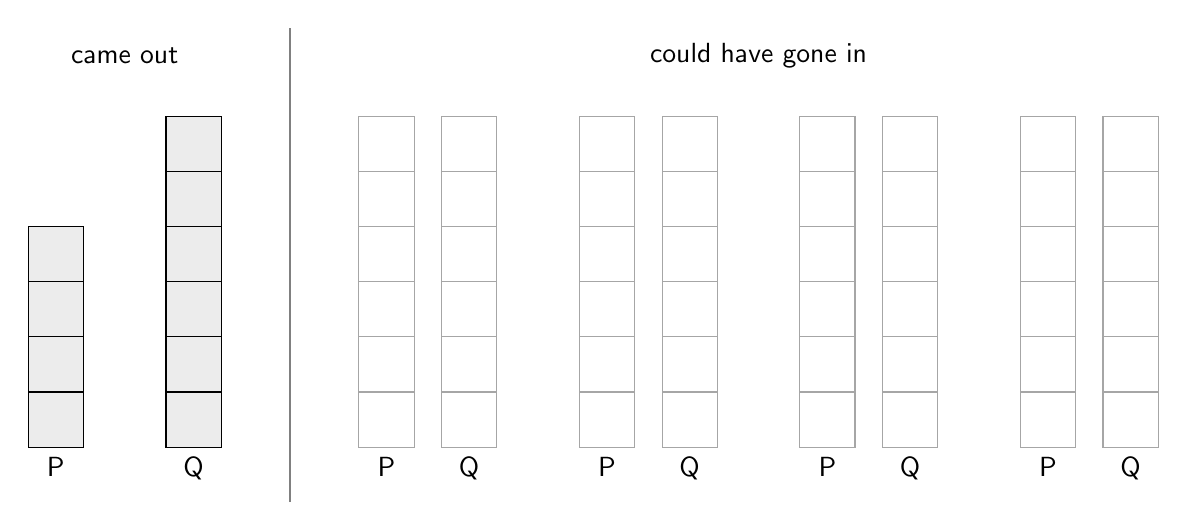
\begin{tikzpicture}[x=7mm,y=7mm]
\node at(1.75,7.1){came out};
\tcubes{0}{0}{4}\node[below]at(.5,0){P};
\tcubes{2.5}{0}{6}\node[below]at(3,0){Q};
\draw[gray](4.75,-1)--(4.75,7.6);
\node at(13.25,7.1){could have gone in};
\foreach\s in{0,...,3}{\tcells{6+4*\s}{0}{6}\node[below]at(6.5+4*\s,0){P};\tcells{7.5+4*\s}{0}{6}\node[below]at(8+4*\s,0){Q};}
\end{tikzpicture}\end{center}

\problem{6}{P and Q still come out as 4 and 6 cubes, but each machine has its own extra. Build P and Q for each machine, and color them.}

\begin{center}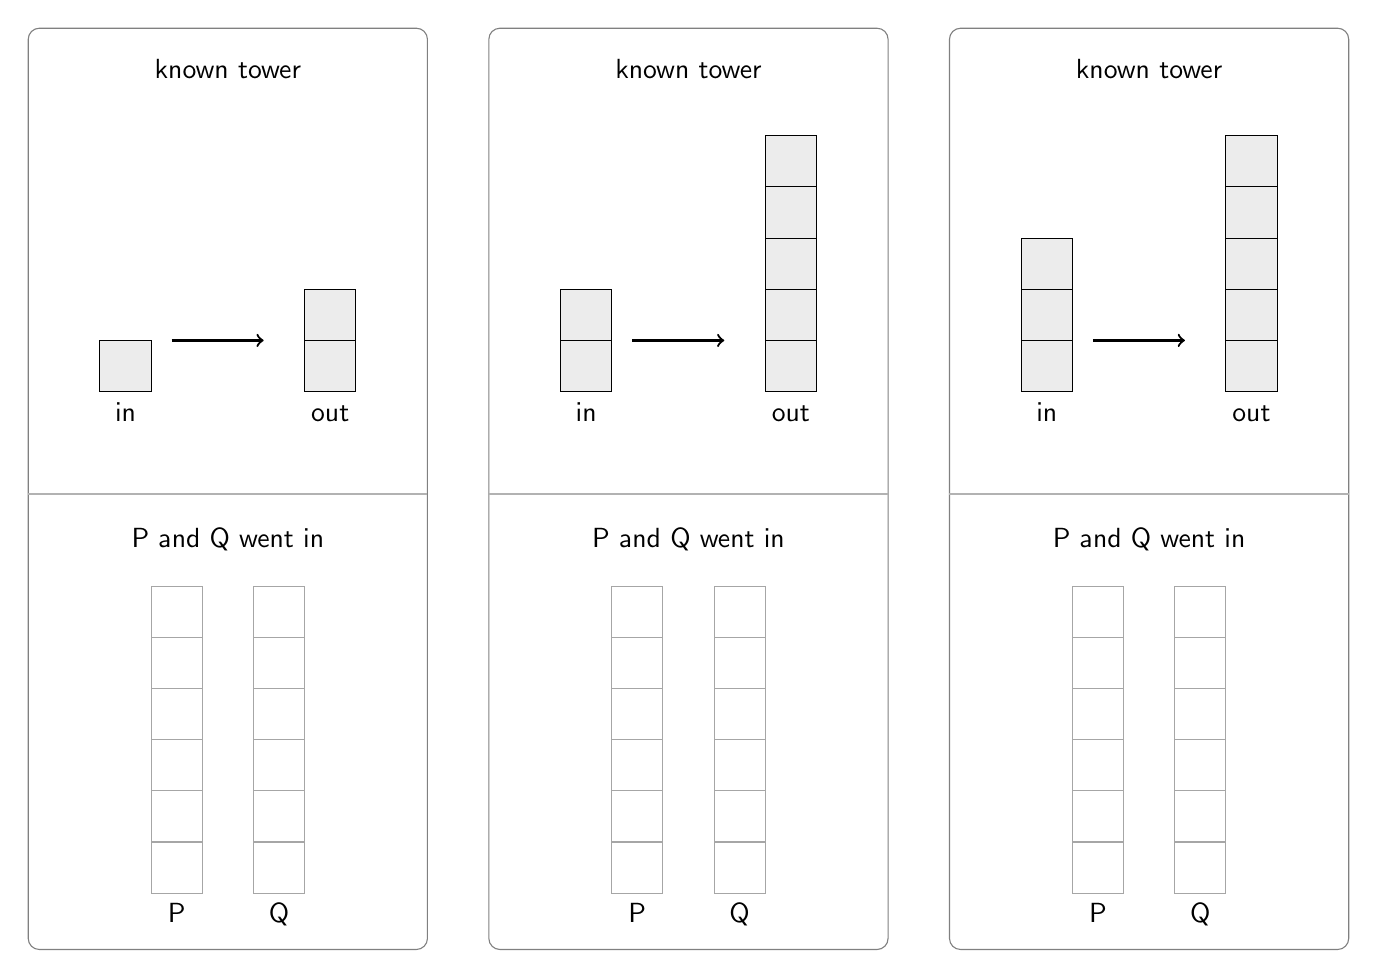
\begin{tikzpicture}[x=6.5mm,y=6.5mm]
\foreach\i/\a/\b in{0/1/2,1/2/5,2/3/5}{\begin{scope}[shift={(9*\i,0)}]
\draw[gray,rounded corners](-1,-10.9)rectangle(6.8,7.1);
\node at(2.9,6.3){known tower};
\tcubes{.4}{0}{\a}\node[below,text height=1.6ex,text depth=.3ex]at(.9,0){in};
\draw[->,thick](1.8,1)--(3.6,1);
\tcubes{4.4}{0}{\b}\node[below,text height=1.6ex,text depth=.3ex]at(4.9,0){out};
\draw[gray!60](-1,-2)--(6.8,-2);
\node at(2.9,-2.9){P and Q went in};
\tcells{1.4}{-9.8}{6}\node[below]at(1.9,-9.8){P};
\tcells{3.4}{-9.8}{6}\node[below]at(3.9,-9.8){Q};
\end{scope}}
\end{tikzpicture}\end{center}
\end{document}
